% Options for packages loaded elsewhere
\PassOptionsToPackage{unicode}{hyperref}
\PassOptionsToPackage{hyphens}{url}
%
\documentclass[
]{book}
\usepackage{lmodern}
\usepackage{amssymb,amsmath}
\usepackage{ifxetex,ifluatex}
\ifnum 0\ifxetex 1\fi\ifluatex 1\fi=0 % if pdftex
  \usepackage[T1]{fontenc}
  \usepackage[utf8]{inputenc}
  \usepackage{textcomp} % provide euro and other symbols
\else % if luatex or xetex
  \usepackage{unicode-math}
  \defaultfontfeatures{Scale=MatchLowercase}
  \defaultfontfeatures[\rmfamily]{Ligatures=TeX,Scale=1}
\fi
% Use upquote if available, for straight quotes in verbatim environments
\IfFileExists{upquote.sty}{\usepackage{upquote}}{}
\IfFileExists{microtype.sty}{% use microtype if available
  \usepackage[]{microtype}
  \UseMicrotypeSet[protrusion]{basicmath} % disable protrusion for tt fonts
}{}
\makeatletter
\@ifundefined{KOMAClassName}{% if non-KOMA class
  \IfFileExists{parskip.sty}{%
    \usepackage{parskip}
  }{% else
    \setlength{\parindent}{0pt}
    \setlength{\parskip}{6pt plus 2pt minus 1pt}}
}{% if KOMA class
  \KOMAoptions{parskip=half}}
\makeatother
\usepackage{xcolor}
\IfFileExists{xurl.sty}{\usepackage{xurl}}{} % add URL line breaks if available
\IfFileExists{bookmark.sty}{\usepackage{bookmark}}{\usepackage{hyperref}}
\hypersetup{
  pdftitle={Notes for: Walsh and Lynch. Genetics and Analysis of Quantitative Traits},
  pdfauthor={Thomas Battram},
  hidelinks,
  pdfcreator={LaTeX via pandoc}}
\urlstyle{same} % disable monospaced font for URLs
\usepackage{longtable,booktabs}
% Correct order of tables after \paragraph or \subparagraph
\usepackage{etoolbox}
\makeatletter
\patchcmd\longtable{\par}{\if@noskipsec\mbox{}\fi\par}{}{}
\makeatother
% Allow footnotes in longtable head/foot
\IfFileExists{footnotehyper.sty}{\usepackage{footnotehyper}}{\usepackage{footnote}}
\makesavenoteenv{longtable}
\usepackage{graphicx}
\makeatletter
\def\maxwidth{\ifdim\Gin@nat@width>\linewidth\linewidth\else\Gin@nat@width\fi}
\def\maxheight{\ifdim\Gin@nat@height>\textheight\textheight\else\Gin@nat@height\fi}
\makeatother
% Scale images if necessary, so that they will not overflow the page
% margins by default, and it is still possible to overwrite the defaults
% using explicit options in \includegraphics[width, height, ...]{}
\setkeys{Gin}{width=\maxwidth,height=\maxheight,keepaspectratio}
% Set default figure placement to htbp
\makeatletter
\def\fps@figure{htbp}
\makeatother
\setlength{\emergencystretch}{3em} % prevent overfull lines
\providecommand{\tightlist}{%
  \setlength{\itemsep}{0pt}\setlength{\parskip}{0pt}}
\setcounter{secnumdepth}{5}

\title{Notes for: Walsh and Lynch. Genetics and Analysis of Quantitative Traits}
\author{Thomas Battram}
\date{2020-06-08}

\begin{document}
\maketitle

{
\setcounter{tocdepth}{1}
\tableofcontents
}
\hypertarget{preface}{%
\chapter*{Preface}\label{preface}}
\addcontentsline{toc}{chapter}{Preface}

This is a good book, but if I make it through the whole thing I deserve several medals and some cake.

\hypertarget{an-overview-of-quantitative-genetics}{%
\chapter{An overview of quantitative genetics}\label{an-overview-of-quantitative-genetics}}

BORWANG!!!

This chapter just introduces the book and some simple concepts.

\hypertarget{properties-of-distributions}{%
\chapter{Properties of distributions}\label{properties-of-distributions}}

ALSO BORWANG!

You can guess what this chapter was on and also how much of a hoot it was\ldots{}

\hypertarget{covariance-regression-and-correlation}{%
\chapter{Covariance, regression, and correlation}\label{covariance-regression-and-correlation}}

\hypertarget{covariance}{%
\section{Covariance}\label{covariance}}

Covariance is a measure of association and the covariance between x and y would be denoted by \(\sigma(x, y)\). If \(x\) and \(y\) are independent then \(\sigma(x, y) = 0\), BUT if \(\sigma(x, y) = 0\), \(x\) and \(y\) aren't necessarily independent.

\hypertarget{useful-identities-for-covariance}{%
\subsection{Useful identities for covariance}\label{useful-identities-for-covariance}}

Covariance of \(x\) with itself = variance of \(x\):

\begin{equation}
    \sigma(x, x) = \sigma^2(x)
    \label{eq:covxx}
\end{equation}

For constants (here represented by \(a\)) see \eqref{eq:cov-rules-contants} below
\begin{align}
    \sigma(a, x) &= 0 \notag \\
    \sigma(ax, y) &= a\sigma(x, y) \notag \\
    \sigma^2(a, x) &= a^2\sigma^2(x) \notag \\
    \sigma[(a + x), y] &= \sigma(x, y) 
    \label{eq:cov-rules-contants}
\end{align}

The covariance of 2 sums can be written as the sum of covariances, i.e.~just multiply out the brackets:

\begin{equation}
  \sigma[(x + y),(w + z)] = \sigma(x, w) + \sigma(x, z) + \sigma(y, w) + \sigma(y, z) 
  \label{eq:cov-of-two-sums}
\end{equation}

Variance of a sum is sum of variances and covariances:

\begin{equation}
  \sigma^2(x + y) = \sigma^2(x) + 2\sigma(x, y) + \sigma^2(y)
  \label{eq:var-of-sum}  
\end{equation}

\hypertarget{least-squares-linear-regression}{%
\section{Least squares linear regression}\label{least-squares-linear-regression}}

Linear model:

\begin{equation}
  y = \alpha + \beta{x} + e
  \label{eq:simple-linear-model}  
\end{equation}

Continuing on, \(\alpha\) and \(\beta\) will be the true population values and \(a\) and \(b\) will be the intercept and slope for the line of best fit derived from observed data. The derivation of \(a\) and \(b\) using the least-squares model can be found on pages 39-41. Buuut, who cares about that, here are the results:

\begin{align}
  a &= \bar{y} - b\bar{x} \notag \\
  b &= \frac{Cov(x, y)} {Var(x)}
  \label{eq:intercept-and-slope}
\end{align}

\hypertarget{properties-of-least-squares}{%
\subsection{Properties of least squares}\label{properties-of-least-squares}}

6 in the book, just writing down important/not obvious ones.

\begin{itemize}
\tightlist
\item
  The mean residual (\(\bar{e}\)) is 0
\item
  Residual errors are uncorrelated with predictor variable \(x\) (see book for why)

  \begin{itemize}
  \tightlist
  \item
    BUT \(e\) and \(x\) may not be independent if the relationship between \(x\) and \(y\) is non-linear. If it is truly non-linear \(E(e|x) != 0\)
  \end{itemize}
\item
  Variance of \(e\) can vary with \(x\), in this situation the the regression is said to display heteroscedasticity (see Figure 3.4 for great illustration)
\item
  The regression of \(y\) on \(x\) is different to the regression of \(x\) on \(y\)!
\end{itemize}

\hypertarget{correlation}{%
\section{Correlation}\label{correlation}}

Correlation coefficient between \(x\) and \(y\):

\begin{equation}
  r(x, y) = \frac{Cov(x, y)} {\sqrt{Var(x) Var(y)}}
  \label{eq:correlation-coef}
\end{equation}

The correlation coefficient is a dimensionless measure of association and it is symmetrical (i.e.~\(r(x, y) = r(y, x)\)).

Scaling \(x\) or \(y\) by constants does not change the correlation coefficient, but it does affect variances and covariances.

The correlation coefficient is a standardised regression coefficient -\textgreater{} the regression coefficient resulting from rescaling \(x\) and \(y\) such that each has unit variance).

\(r^2\) assumes \(E(y|x)\) is linear!

\hypertarget{differential-selection-brief-intro}{%
\section{Differential selection (brief intro)}\label{differential-selection-brief-intro}}

The directional selection differential, \(S\), is the difference between the mean phenotype within that generation before selection (\(\mu_s\)) and the mean phenotype within that generation after (\(\mu\)) selection.

\begin{equation}
  S = \mu_s - \mu
  \label{eq:selection-differential}
\end{equation}

If all individuals have equal fertility and viability then selecting individuals won't change anything so \(\mu_s = \mu\) and \(S = 0\).

If \(W(z)\) is the probability that individuals with phenotype \(z\) survive to reproduce and \(p(z)\) is the density of \(z\) (pretty much means distribution) before selection, then the density after selection is:

\begin{equation}
  p_{s}(z) = \frac{W(z)p(z)} {\int W(z)p(z)dz}
  \label{eq:density-after-selection}
\end{equation}

The denominator here is the mean individual fitness (\(\bar{W}\)). The relative fitness of \(z\) is \(w(z) = \frac{W(z)} {\bar{W}}\).

After some sweet derivation (see page 46), you finish with:

\begin{equation}
  S = \sigma[z, w(z)]
  \label{eq:selection-differential2}
\end{equation}

Therefore the directional selection is equivalent to the covariance of the phenotype and the relative fitness.

If you regress offspring phenotype on the midparent phenotype and that relationship is linear with slope \(\beta\), a change in mean midparent phenotype induces an expected change in mean phenotype across generations equal to:

\begin{equation}
\begin{split}
  \Delta\mu &= \mu_0 - \mu \\
  &= \beta(\mu_s - \mu) \\
  &= \beta{S}
\end{split}
\label{eq:breeders-equation}
\end{equation}

This is the breeders' equation!

\hypertarget{correlation-between-genotype-and-phenotype-brief-intro}{%
\section{Correlation between genotype and phenotype (brief intro)}\label{correlation-between-genotype-and-phenotype-brief-intro}}

Only when there is no gene-environment interaction is the variance explained by genetics (broad-sense heritability) the equation below:

\begin{equation}
  H^2 = \frac{\sigma^2_G} {\sigma^2_z},
  \label{eq:broad-sense-heritability}
\end{equation}

where \(z\) is the phenotype and \(G\) is the sum of the total effects (not just additive) at all loci on the trait.

The slope of a midparent-offspring regression provides an estimate of the proportion of the phenotypic variance that is attributable to additive genetic factors (the narrow-sense heritability).

\begin{equation}
  h^2 = \frac{\sigma^2_A} {\sigma^2_z}
  \label{eq:narrow-sense-heritability}
\end{equation}

So as \(h^2\) is just the regression of offspring phenotype on midparent phenotype it can actually be used in the breeders' equation!

\begin{equation}
  \Delta\mu = h^2S
  \label{eq:breeders-equation-with-h2}
\end{equation}

So the narrow-sense heritability can be thought of as the efficiency of the response to selection. If \(h^2 = 0\) there can be no evolutionary change regardless of strength of selection. Although this should be obvious because if \(h^2\) is 0 then there is clearly no passing of genetic material onto the next generation that is influencing that trait.

\hypertarget{end-of-chapter-questions}{%
\section{End of chapter questions}\label{end-of-chapter-questions}}

\begin{enumerate}
\def\labelenumi{\arabic{enumi}.}
\tightlist
\item
  True or false, if \(\sigma(x,y) = 0\), \(x\) and \(y\) are independent
\item
  Finish these equations:
  \begin{align}
    \sigma[(x + y),(w + z)] &= ... \notag \\
    \sigma^2(a, x) &= ... \notag \\
    \sigma[(a + x), y] &= ... \notag \\
    \sigma^2(x + y) &= ... \notag \\
  \end{align}
\item
  Give 2 properties of residuals from least-squares regression
\item
  What is heteroscedasticity?
\item
  True or false, \(y\) \textasciitilde{} \(x\) will always give the same effect estimate as \(x\) \textasciitilde{} \(y\)
\item
  Give an assumption of the correlation coefficient
\item
  How can you work out \(h^2\) from trio data?
\item
  Give two definitions of the breeders' equation.
\end{enumerate}

\hypertarget{properties-of-single-loci}{%
\chapter{Properties of single loci}\label{properties-of-single-loci}}

\hypertarget{introduction}{%
\section{Introduction}\label{introduction}}

too easy

\hypertarget{allele-and-genotype-frequencies}{%
\section{Allele and genotype frequencies}\label{allele-and-genotype-frequencies}}

too easy

\hypertarget{the-transmission-of-genetic-information}{%
\section{The transmission of genetic information}\label{the-transmission-of-genetic-information}}

\hypertarget{the-hardy-weinberg-principle}{%
\subsection{The Hardy-Weinberg principle}\label{the-hardy-weinberg-principle}}

\begin{equation}
  p^2 + 2pq + q^2 = 1
  \label{eq:hardy-weinberg-principal}
\end{equation}

where \(p\) = allele frequency of first allele at a locus and \(q\) = allele frequency of the second allele at that same locus.

Assumptions of H-W:

\begin{itemize}
\tightlist
\item
  No selection
\item
  No mutation
\item
  Random mating
\item
  No differential migration
\item
  No random drift
\end{itemize}

Even though these assumptions will never be met completely in the real world, for the majority of the time the H-W prinicple holds regardless.

Assuming assumptions are met, 2 important points from H-W:

\begin{enumerate}
\def\labelenumi{\arabic{enumi}.}
\tightlist
\item
  It takes no more than a single generation to equilibriate and stabilize gene frequencies in the two sexes.
\item
  Only one additional generation is required for the stabilisation of the genotype frequencies into the predictible Hardy-Weinberg proportions.
\end{enumerate}

\hypertarget{sex-linked-loci}{%
\subsection{Sex-linked loci}\label{sex-linked-loci}}

Alleles on sex chromosomes in diploid organisms are obviously different. Sons can only receive an X chromosome from their mother so the frequency of X linked loci in the sons is equal to that of their mothers. Daughters receive both an X chromosome from Mum + from Dad.

Overall this means allele frequencies oscilate around an equilibrium state, but continually get closer to that state over the generations (see Figure 4.2 and page 56 for equation).

\hypertarget{polyploidy}{%
\subsection{Polyploidy}\label{polyploidy}}

Skipped over this section because it's not relevant to human quant gen. Buuut, essentially it just details how to derive allele frequencies under a certain case of polyploidy. Also, it should be noted that of course H-W does not hold under polyploidy!

\hypertarget{age-structure}{%
\subsection{Age structure}\label{age-structure}}

Age structure also complicates our idealised model of H-W. In populations composed of several age classes, the generations overlap, and this causes the approach of genotype frequencies towards the H-W expectations to be gradual (rather than just by 1 or 2 generations), even in the case of an autosomal locus. Doesn't explain this very much, but it's covered elsewhere. Importantly, when newly founded populations have significant age structure, fluctuations in both gene and genotoype frequencies may occur for a substantial period of time even in the abscence of selection!

\hypertarget{testing-for-hardy-weinberg-proportions}{%
\subsection{Testing for Hardy-Weinberg proportions}\label{testing-for-hardy-weinberg-proportions}}

Says in the book that LRT can be used to test for departures from HWE and it can, but another common method is the chi-squared test and in \href{https://www.cog-genomics.org/plink/1.9/}{PLINK} they used Haldane's exact test which is apparently analogus to Fisher's exact test (\href{https://www.genetics.org/content/183/4/1431}{papier on it}) (can also use Fisher's exact test if the sample size is tiny and the allele is rare.). Essentially, in a population, at a specific locus, you can calculate the allele frequencies (and from that expected genotype frequencies) from the observed genotype frequencies then test if there is a difference between the observed and expected values. LRT equation for it given on page 60. See code for some comparisons.

Should remember (as pointed out above), that just because some assumptions are violated, doesn't mean you'd get a departure from HWE!

\hypertarget{characterising-the-influence-of-a-locus-on-the-phenotype}{%
\section{Characterising the influence of a locus on the phenotype}\label{characterising-the-influence-of-a-locus-on-the-phenotype}}

If a trait is entirely influenced by a single locus then the genetic effect on that trait can be characterised pretty easily and the dominance and additive effects of the alleles can be calculated. So if a locus has genotypes \(B_1B_1\), \(B_1B_2\), \(B_2B_2\), then the values given to these genotypes can be said to be: \(-a\), \((1 + k)a\) and \(+a\). Now if you have genotype data at that locus and data on the trait you can work out the effect of the \(B_2\) allele by taking the mean phenotypic value of individuals with \(B_2B_2\) and subtracting the mean phenotypic value of individuals with \(B_1B_1\) and dividing by 2 i.e.

\begin{equation}
  B_{2eff} = \frac{p_{B2} - p_{B1}} {2}
  \label{eq:effect-of-b2}
\end{equation}

where \(B_{2eff}\) is the effect of allele \(B_2\), \(p_{B2}\) is the mean phenotypic value of individuals with \(B_2B_2\) and \(p_{B1}\) is the mean phneotypic value of individuals with \(B_1B_1\).

As \(B_{2eff} = a\) you can then substitute this in to \((1 + k)a\) to get the dominance coefficient \(k\). Of course if \(k = 0\) then there is no dominance (in reality you would calculate probability of dominance).

\hypertarget{the-basis-of-dominance}{%
\section{The basis of dominance}\label{the-basis-of-dominance}}

Confusing part\ldots{} Don't really get the enzyme activity bit\ldots{}

Main point (I think) is that new deleterious mutations are very likely to be recessive and new mutations with a slight deleterious effect interact in an almost entirely additive fashion (no dominance!).

\hypertarget{fishers-decomposition-of-the-genotypic-value}{%
\section{Fisher's decomposition of the genotypic value}\label{fishers-decomposition-of-the-genotypic-value}}

Recalling that the phenotypic value can be partitioned like so:

\begin{equation}
  z = G + E
  \label{eq:phenotypic-value-partition}
\end{equation}

where \(z\) is the phenotype, \(G\) is the genotypic value and \(E\) is the environmental value.

The genotypic value of a specific locus can be partitioned into it's ``expected'' values based on there being only additive effects (\(\hat{G}\)) and the deviations from the expected values or dominance effects (\(\delta\)). So for genotype \(B_iB_j\):

\begin{equation}
  G_{ij} = \hat{G_{ij}} + \delta_{ij}
  \label{eq:expected-genotypic-value-simple}
\end{equation}

This can be formalised (whatever the fuck that means) by regressing the genotypic values on the number of \(B_1\) and \(B_2\) alleles in the genotype (\(N_1\) and \(N_2\)):

\begin{equation}
  G_{ij} = \hat{G_{ij}} + \delta_{ij} = \mu_G + \alpha_1N_1 + \alpha_2N_2
  \label{eq:expected-genotypic-value-2}
\end{equation}

\(\mu_G\) = the mean genotypic value in the population, \(\alpha_1\) and \(\alpha_2\) are the slopes of the regression, \(N_1\) and \(N_2\) are the number of \(B_1\) and \(B_2\) alleles. So the regression is:

\begin{equation}
  G_{ij} ~ N_2 + N_1
\end{equation}

By noting that for any individual, \(N_1 = 2 - N_2\) you can reduce the multiple regression model into an easier to work with univariate model. Give it a go (use equation \eqref{eq:expected-genotypic-value-2}):

\begin{equation}
\begin{split}
  G_{ij} &= \mu_G + \alpha_1(2 - N_2) + \alpha2N_2 + \delta_{ij} \\
  &= l + (\alpha_2 - \alpha_1)N_2 + \delta_{ij}
\end{split}
\label{eq:genotypic-value-regression}
\end{equation}

where \(l = \mu_G + 2\alpha_1\) is the intercept and the slope is \(\alpha = \alpha_2 - \alpha_1\)

If you plotted the genotypic value (\(G\)) against gene content (\(N_2\) or number of \(B_2\) alleles) and calculated residuals these residuals would be \(\delta\), the dominance deviation (see Figure 4.6).

The rest of the chapter uses this regression and what we know about genotype frequencies to derive a formula for the average effect of allelic substitution:

\begin{equation}
  \alpha = a[1 + k(p_1 - p_2)]
  \label{eq:allelic-sub-effect}
\end{equation}

where \(a\) = genotypic value of \(B_2\) (see above), \(k\) is the dominance coefficient and \(p_1\) and \(p_2\) are the frequencies of \(B_1\) and \(B_2\). This value \(\alpha\) represents the average change in genotypic value that results when a \(B_2\) allele is randomly substituted for a \(B_1\) allele. If no dominance (\(k = 0\)) then \(\alpha = a\). Except in the case of additivity, the average effect of allelic substitution is not simply a function of the inherent physiological properties of the allele. It can only be defined in the context of the population!

\hypertarget{partioning-the-genetic-variance.}{%
\section{Partioning the genetic variance.}\label{partioning-the-genetic-variance.}}

Deriving variance of \(G\):

\begin{align}
\begin{split}
  G &= \hat{G} + \delta \notag \\
  \sigma^2_G &= \sigma^2(\hat{G} + \delta) \notag \\
  &= \sigma^2(\hat{G}) + 2\sigma(\hat{G} + \delta) + \sigma^2(\delta)
\end{split}
\label{eq:total-genetic-variance-longwinded}
\end{align}

The top equation is just like a regression, with \(\delta\) being the residual error and we know that for least-squares there is no correlation between the residual error and the predictor. So there is no correlation between \(\hat{G}\) and \(\delta\). Therefore:

\[ \sigma^2_G = \sigma^2(\hat{G}) + \sigma^2(\delta) \]
OR more commonly
\begin{equation}
  \sigma^2_G = \sigma^2_A + \sigma^2_D
  \label{eq:genetic-variance-one-locus}
\end{equation}

\(\sigma^2_A\) is the variance of \(G\) explained by regression on \(N_2\) (or \(N_1\)), and \(\sigma^2_D\) is the residual variance of that regression. The variance of the additive and dominance effects!

For a diallelic locus we can do some rearranging of equations in Table 4.1 of the book and get these equations:

\begin{align}
  \sigma^2_A &= 2p_1p_2\alpha^2 \label{eq:additive-var} \\
  \sigma^2_D &= (2p_1p_2ak)^2 \label{eq:dominance-var}
\end{align}

From these we can clearly see that both components depend on allele frequencies, the dominance coefficient and the homozygous effect (remember \(\alpha\) is just the slope of the \(G ~ N_2\) regression!).

By plotting how genetic variance changes with gene frequency under different scenarios (see \ref{fig:sigma-g-gene-frequency}). You see some interesting patterns. Firstly, at a single diallelic locus, you see that \(\sigma^2_A\) reaches it's peak when \(p_1 = p_2 = 0.5\). Secondly, it's clear that, even in the case of overdominance (which is rare!), additive genetic variance will almost always be much higher than genetic variance from dominance effects, even when the frequency of the dominant allele is high.



\begin{figure}
\centering
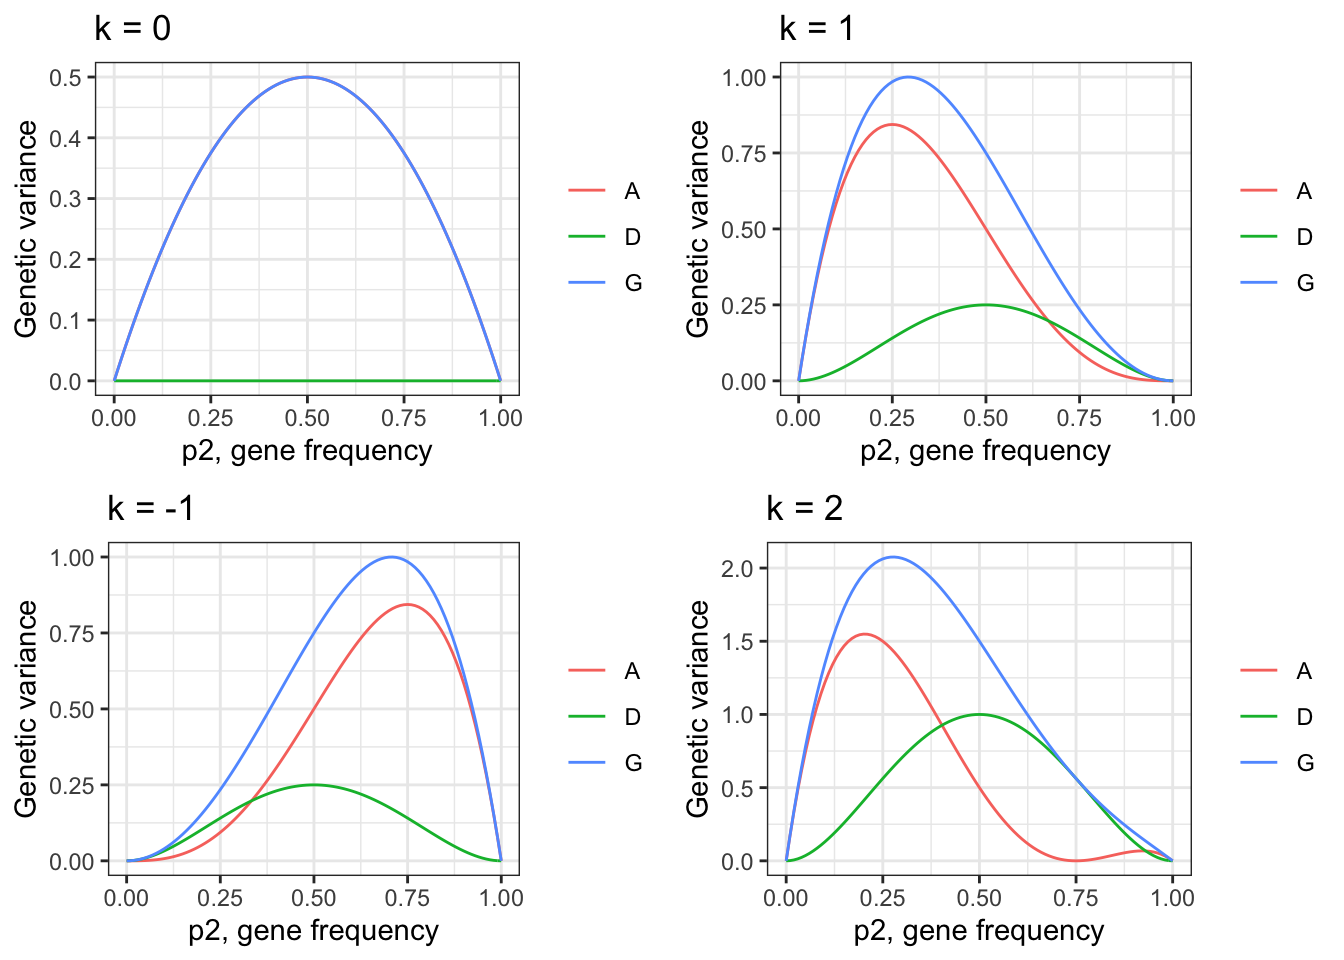
\includegraphics{quant_genetics_book_notes_files/figure-latex/sigma-g-gene-frequency-1.pdf}
\caption{\label{fig:sigma-g-gene-frequency}The dependence of components of genetic variance at a locus on the frequency of the \(B_2\) allele. \(a\) is set to be one, which scales the vertical axes so that for any particular case, the actual variances are obtainable by multiplying by \(a^2\).}
\end{figure}

\hypertarget{additive-effects-average-excesses-and-breeding-values}{%
\section{Additive effects, average excesses and breeding values}\label{additive-effects-average-excesses-and-breeding-values}}

The dominance deviation of a parent, which is a function of the interaction between the two parental alleles, is eliminated when gametes are produced. Thus, one can think of \(\hat{G}\) and \(\delta\) as the heritable and nonheritable components of an individual's genotypic value.

Fisher proposed two different measures of the effect of an allele: one being the additive effect (\(\alpha_i\)) and then the average excess \(\alpha^x_i\). The average excess \(\alpha^x_2\) of allele \(B_2\) is the difference between the mean genotypic value of individuals carrying at least one copy of \(B_2\) and the mean genotypic value of a random individual from the entire population:

\begin{equation}
  \alpha^x_2 = (G_{12}P_{12|2} + G_{22}P_{22|2}) - \mu_G
  \label{eq:average-excess-effect}  
\end{equation}

where \(P_{ij}\) is the conditional probability of a \(B_iB_j\) genotype given that one allele is \(B_i\). Under random mating \(P_{ij|i} = p_j\) (\(p_j\) = frequency of allele \(B_j\)). THINK ABOUT HARDY-WEINBERG AND IT MAKES SENSE!

So under random mating,

\begin{equation}
  \alpha^x_2 = G_{12}p_1 + G_{22}p_2 - \mu_G
  \label{eq:average-excess-effect2}
\end{equation}

\(G_{12} = a(1+k)\) and \(G_{22} = 2a\). By substituting these into the equation above for \(\alpha^x_1\) and \(\alpha^x_2\) and then calculating \(\alpha_1\) and \(\alpha_2\) (additive effects) by the method previously mentioned (regressing genotypic value \(G\) on the number of \(B_2\) alleles, \(N_2\)), we will see they're equivalent (shown on page 72):

\begin{align}
  \alpha_2 &= p_1\alpha \notag \\
  \alpha_1 &= -p_2\alpha
\end{align}

The breeding value of an individual (\(A\)) is the sum of the additive effects of its genes. So the breeding value of a \(B_1B_1\) homozygote is just \(2\alpha_1\). In randomly mating populations the breeding value of a genotype is equivalent to twice the expected deviation of its offspring mean phenotype from the population mean. Soooo, no genotype information is needed to calculate the breeding value. All we have to do is mate an individual to many randomly chosen individuals from the population and taking twice the deviation of its offspring mean from the population mean. EASY IN HUMANS!!!

In Chapter 13 this will be discussed wrt candidate gene studies.

\hypertarget{extensions-for-multiple-alleles-and-non-random-mating}{%
\section{Extensions for multiple alleles and non random mating}\label{extensions-for-multiple-alleles-and-non-random-mating}}

So this section seems mostly unrelevant as we're unlikely to deal with situations with more than 2 alleles. Non-random mating could be encountered if we're interested in some phenotypes (e.g.~alcohol intake). Buuuut, it's still good to note some of the generalised equations for what we've been discussing so far in the chapter.

\hypertarget{average-excess}{%
\subsection{Average excess}\label{average-excess}}

When \(n\) alleles are present, the average excess, \(\alpha^x_i\), for any allele \(B_i\) is given by

\begin{equation}
  \alpha^x_i = \sum_{j=1}^{n} P_{ij|i}G_{ij} - \mu_G
  \label{eq:average-excess-effect3}
\end{equation}

Remember, under random mating \(P_{ij|i} == p_j\)

\hypertarget{additive-effects}{%
\subsection{Additive effects}\label{additive-effects}}

The genotypic value can also be obtained using regression as before, but in it's generalised form is a multivariate regression. For \(n\) alleles

\begin{equation}
  G = \mu_G + \sum_{i=1}^{n} \alpha_{i}N_{i} + \delta
  \label{eq:generalised-genotypic-value-regression}
\end{equation}

After some re-arranging can derive the regression coefficients and finally end with

\begin{equation}
  \alpha_i = \sum_{j=1}^{n} p_jG_{ij} - \mu_G
  \label{eq:all-average-effects}
\end{equation}

i.e.~under random mating, the average effects (\(\alpha_i\)) are equal to the conditional mean deviations from the mean genotypic value of the population (\(\mu_G\)).

For non-random mating we need the inbreeding coefficient, \(f\) to define our genotype frequencies:

\begin{align}
  P_{ii} &= (1 - f)p^2_i + fp_i \notag \\
  P_{ij} &= 2(1 -f)p_ip_j
  \label{eq:nonrandom-mating-genotype-frequencies}
\end{align}

Unsure of why, but this means

\begin{equation}
  \alpha_i = \frac{\alpha^x_i} {1 + f}
  \label{eq:average-effects-inbreeding}
\end{equation}

so \(f\) is the fractional reduction of heterozygote frequencies relative to those expected under random mating. This means you can kind of do a test for random mating by checking heterozygote and homozygote frequencies in a population!

\hypertarget{additive-genetic-variance}{%
\subsection{Additive genetic variance}\label{additive-genetic-variance}}

The additive genetic variance across \(n\) alleles is

\begin{equation}
  \sigma^2_A = 2 \sum_{i=1}^{n} p_i\alpha_i\alpha^x_i
  \label{eq:all-additive-genetic-variance}  
\end{equation}

In general inbreeding inflates the additive genetic variance by causing correlations among the effects of alleles within the same individuals.

The broad sense heritability, even under scenarios of non-random mating can be given by

\begin{equation}
  \sigma^2_G = \sigma^{2}(\alpha_i + \alpha_j) + \sigma^{2}(\delta_{ij})
\end{equation}

although it should be noted that the definitions of \(\alpha_i\) and \(\delta_ij\) change with the degree of inbreeding! Random mating means \(\alpha_i\) and \(\alpha_j\) are uncorrelated so we get back to the good old equation

\[ \sigma^2_G = \sigma^2_A + \sigma^2_D \]

Importantly, under random mating, \(\sigma^2_A\) is equivalent to the variance of breeding values of individuals in the population.

\begin{center}\rule{0.5\linewidth}{0.5pt}\end{center}

\textbf{Summarising some key terms}

\textbf{The homozygous effect, \(a\), and the dominance coefficient, \(k\),} are intrinsic properties of allelic products. They are not functions of allele frequencies, but may vary with genetic background

\textbf{The additive effect, \(\alpha_i\), and the average excess, \(\alpha^x_i\),} are properties of alleles in a particular population. They are functions of \(a\), \(k\) and genotype frequencies (\(p_i\)).

\textbf{The breeding value, \(A\),} is a property of a particular individual in reference to a particular population. It's equivalent to the sum of the additive effects of an individual's alleles.

\textbf{The additive genetic variance, \(\sigma^2_A\)} is a property of a particular population. It is equivalent to the variance of the breeding values of individuals within the population.

\begin{center}\rule{0.5\linewidth}{0.5pt}\end{center}

\hypertarget{end-of-chapter-questions-1}{%
\section{End of chapter questions}\label{end-of-chapter-questions-1}}

\begin{enumerate}
\def\labelenumi{\arabic{enumi}.}
\tightlist
\item
  What is the Hardy-Weinberg principle and what are it's assumptions?
\item
  What does the H-W principle mean for gene and genotype frequencies across generations?
\item
  What is age structure and how does it affect HWE?
\item
  How can you test for HWE?
\item
  Are deliterious mutations likely to be dominant or recessive?
\item
  Assuming a trait was entirely influenced by a single locus, how could you calculate dominance and additive effects knowing the genotypes and phenotypes of the individuals in the sample?
\item
  What is the formula for the average effect of allelic substitution?
\item
  For a diallelic locus, what does the additive genetic variance and dominance genetic variance depend on?
\item
  How does the contribution of additive genetic variance to total genetic variance change when \(k\) varies?
\item
  What is the breeding value of an individual?
\item
  Define the additive genetic variance in the presence of \(n\) alleles
\item
  Learn the definitions of the key terms!
\end{enumerate}

\hypertarget{sources-of-genetic-variation-for-multilocus-traits}{%
\chapter{Sources of genetic variation for multilocus traits}\label{sources-of-genetic-variation-for-multilocus-traits}}

\hypertarget{epistasis}{%
\section{Epistasis}\label{epistasis}}

Epistasis describes the nonadditivity of effects between loci, i.e.~the alleles of one loci influence the effects of another loci.

The genotypic value, \(G_{ijkl}\), needs to take into account all the interaction terms that can arrive between loci, for two loci it's additive x additive effects (\(\alpha\alpha\)), additive x dominance effects (\(\alpha\delta\)), and dominance x dominance effects (\(\delta\delta\)). As the number of loci increases the number of interaction terms increase steadily e.g.~\(\alpha\alpha\alpha\) will be there for three loci.

\hypertarget{a-general-least-squares-model-for-genetic-effects}{%
\section{A general least-squares model for genetic effects}\label{a-general-least-squares-model-for-genetic-effects}}

This is just an extension of the one-locus linear model introduced in Chapter 4.

For this section, imagine we are interested in measuring the genetic effects of two loci, \(G_{ijkl}\), which can easily be extended to more. The additive effect of an allele on a phenotype is just the phenotypic value in people with that allele minus the mean phenotypic value of the population. When considering epistatic effects we can define it in the same way.

\begin{equation}
  \alpha_{i} = G_{i...} - \mu_{G}
  \label{eq:additive-effects-i}
\end{equation}

\(G_{i...}\) is just the conditional mean phenotype of individuals with allele \(i\) at the first locus without regard to the other allele at that locus or to the genotype at the second locus. The other additive terms (for \(\alpha_{j}\), \(\alpha_{k}\), \(\alpha_{l}\)) are defined in the same way. Within each locus, the mean value of average effects (weighted by allele frequency) = 0.

Dominance effects can be defined in a similar way, complete these equations by recalling \eqref{eq:generalised-genotypic-value-regression}:

\begin{align}
  \delta_{ij} &= G_{ij..} - ... \label{eq:dom-effects-ij} \\
  \delta_{lk} &= G_{..lk} - ... \label{eq:dom-effects-lk}
\end{align}

Like with the additive effects, the mean dominance deviation at each locus is equal to zero.

Epistatic effect terms proceed in a similar fashion. Letting \(G_{i.k.}\) be the mean phenotype of individuals with gene \(i\) at locus 1 and \(k\) at locus 2, without regard to the other two genes, the \(ik\)th additive x additive effect is:

\begin{equation}
  \left(\alpha\alpha\right)_{ik} = G_{i.k.} - \mu_{G} - \alpha_{i} - \alpha_{k} 
  \label{eq:add-add-effects-ik}
\end{equation}

So \(\left(\alpha\alpha\right)_{ik}\) is the deviation of the conditional mean \(G_{i.k.}\) from the expectation based on the population mean \(\mu_{G}\) and the additive effects \(\alpha_{i}\) and \(\alpha_{k}\). An additive x dominance effect measures the interaction between an allele at one locus with a genotype of another locus (see equation 5.5 in book) and the dominance x dominance effect involves an interaction between the genotypes at each locus (see equation 5.6 in book).

\begin{equation}
  TO DO
  \label{eq:complete-genotypic-value}
\end{equation}

The complete genotypic value, \(G_{ijkl...}\) can be found in equation 5.7 in the book. These parameters depend on genotype frequencies in the population, but the mean value of each type of effect is always equal to zero.

The genotypic value of an individual is often impossible to quantify because of variation in the phenotype due to the environment, but the genotypic value for an individual equation can be extended to populations. Providing mating is random and segregation of loci is independent, there is no statistical relationship between the genes found within or among loci. So the total genetic variance is just the sum of the variance of the individual effects, simplified this is:

\begin{equation}
  \sigma^{2}_{G} = \sigma^{2}_{A} + \sigma^{2}_{D} + \sigma^{2}_{AA} + \sigma^{2}_{AD} + \sigma^{2}_{DD} + ...
  \label{eq:multilocus-genetic-variance}
\end{equation}

\ldots{} here and in other cases just symbolises more terms can be added if more than two loci are used.

Epistatic effects are expected to be common throughout the genome and Wright thought they were the rule, rather than exception. See example two in the book for calculations of epistatic effects and how much variance they contribute to the overall genetic variance component. Overall, it is clear that even with large epistatic effects, additive genetic variance, \(\sigma^{2}_{A}\) will pretty much always (if not always) contribute to the vast majority of overall genetic variance \(\sigma^{2}_{G}\). This is important for two reasons:

\begin{enumerate}
\def\labelenumi{\arabic{enumi}.}
\tightlist
\item
  Variance components provide limited insight into the physiological mode of gene action, i.e.~just because genetic variance is explained by additive effects (which means you essentially count each gene separately), it does not mean the interaction between genes is not important in terms of their function!
\item
  When interested in the variance of a trait that is explained by genetics, you can expect the vast majority of that variance to be explained by additive genetic effects, which makes things like estimating heritability far easier.
\end{enumerate}

\hypertarget{extension-to-haploids-and-polyploids}{%
\subsection{Extension to haploids and polyploids}\label{extension-to-haploids-and-polyploids}}

Skipped this section as not relevant to humans.

\hypertarget{linkage}{%
\section{Linkage}\label{linkage}}

Genes of the same chromosome tend to be inherited as a group, a tendency that declines with increasing distance between the loci. Crossing-over during meiosis is responsible for this decline.

\begin{center}\rule{0.5\linewidth}{0.5pt}\end{center}

\textbf{Difference between linkage and linkage disequilibrium}

Loci are linked if they tend to be inherited together. If loci are correlated for any reason (don't need to be inherited together), they are in linkage disequilibrium. The census units for measuring linkage are gamete frequencies, so you can use an individual to estimate this. LD is measured across a population.

Can get linkage without LD, can get linkage and LD, and can get two correlated loci (LD) that aren't linked.

\begin{center}\rule{0.5\linewidth}{0.5pt}\end{center}

Even though you can get correlated loci for reasons other than linkage, the LD between linked loci are more likely to persist over time as seen in \eqref{eq:LD-decay}.

Under linkage equilibrium, the frequency of gametes is the product of allele frequencies, so for loci \(A\) and \(B\),

\begin{equation}
  Freq(AB) = Freq(A) * Freq(B)
  \label{eq:linkage-equilibrium}
\end{equation}

So A and B are independent of each other.

Measure of disequilibrium is just the departure from this:

\begin{equation}
  D_{AB} = Freq(AB) - Freq(A) * Freq(B)
  \label{eq:LD-D}
\end{equation}

\(D_{AB}\) can be positive or negative depending on whether \(A\) and \(B\) are in coupling (\(AB\) gametes are overrepresented) or repulsion (\(AB\) gametes are underrepresented) disequilibrium. \(D\) is often referred to as the coefficient of linkage disequilibrium (although can be non-zero without linkage!).

Selection, migration, mutation and drift can help maintain LD. Even without these forces, once LD is established it can be maintained for many generations (especially if loci are more tightly linked!).

Expected LD changes over time depend on the recombination fraction between loci, \(c\). This value ranges from 0 to 0.5, where 0 essentially means the loci are inherited together and 0.5 is free recombination between loci.

If recombination frequency between the \(A\) and \(B\) loci is \(c\), the disequilibrium in generation \(t\) is given by:

\begin{equation}
  D(t) = (1 - c)^{t}D(0)
  \label{eq:LD-decay}
\end{equation}

This equation is graphically displayed in \ref{fig:ld-decay}.



\begin{figure}
\centering
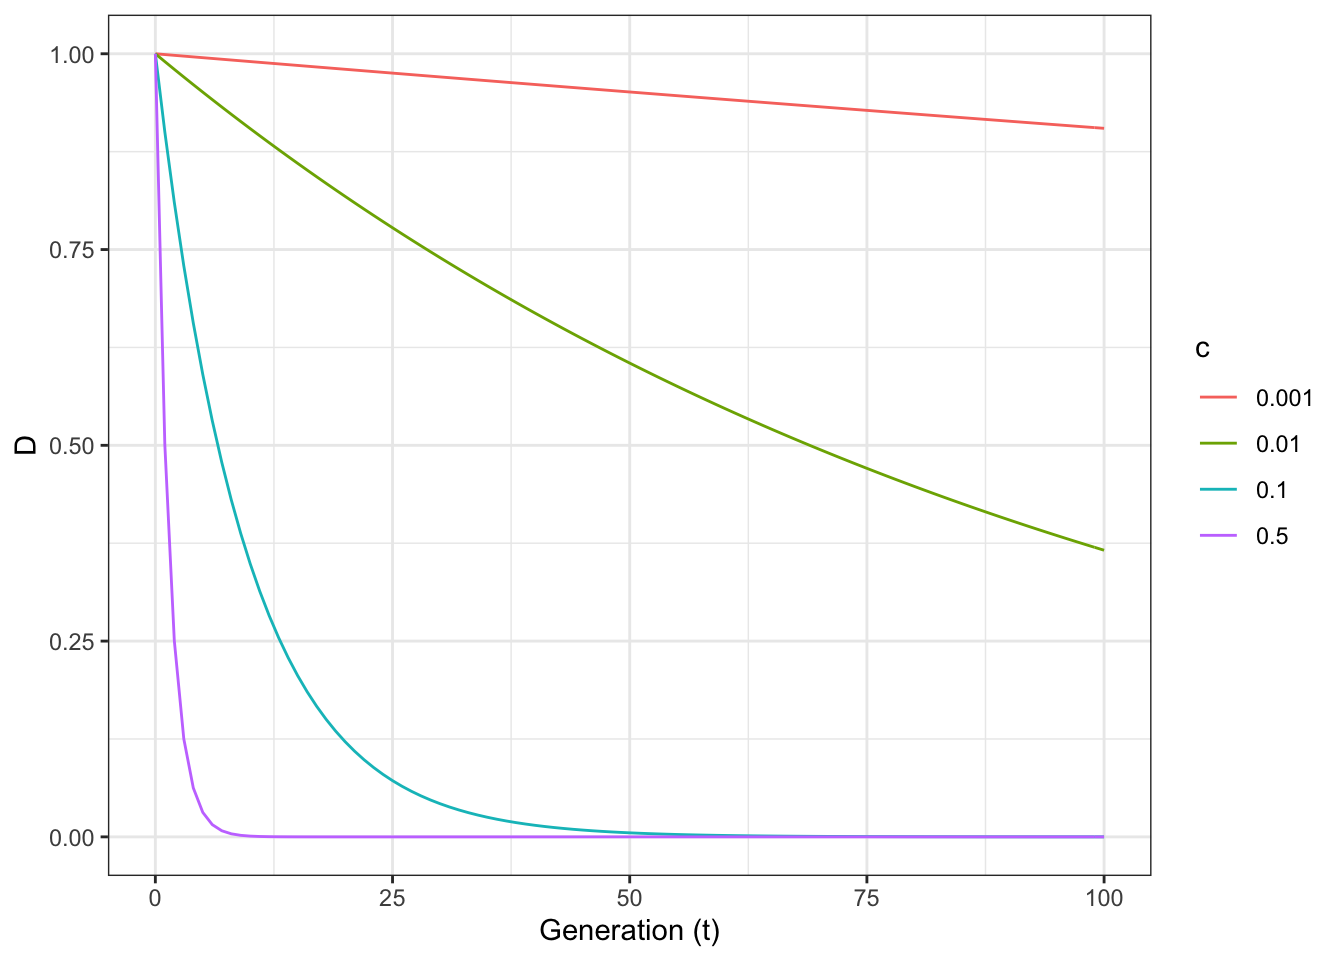
\includegraphics{quant_genetics_book_notes_files/figure-latex/ld-decay-1.pdf}
\caption{\label{fig:ld-decay}The decline, under random mating, of linkage disequilibrium when the initial value {[}D(0){]} is set to 1 as a function of the recombination frequency, c.}
\end{figure}

To estimate \(D\) you can directly count gamete frequencies of an individual. This is not possible for most organisms though and usually you have to make-do with measured multilocus genotypes across a population. You can then workout gametes used to produce the genotypes (e.g.~someone with an \(AABb\) genotype would be formed from a \(AB\) gamete and \(aB\) gamete). However, with double heterozygotes you can't be sure if an \(ABab\) individual was formed from \(AB\) and \(ab\) gametes or from \(Ab\) and \(aB\) gametes. Under random mating, it's not necessary to distinguish between coupling and repulsion heterozygotes so this doesn't really matter. In this case an estimate of \(D\) is given by:

\begin{equation}
  \hat{D_{AB}} = \frac{N} {N - 1} [\frac{4N_{AABB} + 2(N_{AABb} + N_{AaBB}) + N_{AbBb}} {2N} -2\hat{p_{A}}\hat{p_{B}}]
  \label{eq:LD-from-genotypes}
\end{equation}

The equation for the sampling variance of \(D\) is shown on page 99.

Ideally you'd have 1000s of samples to achieve reasonable statistical power when estimating \(D\) using multilocus genotype frequencies.

\hypertarget{effect-of-disequilibrium-of-the-genetic-variance}{%
\section{Effect of disequilibrium of the genetic variance}\label{effect-of-disequilibrium-of-the-genetic-variance}}

The aggregate effects of gametic phase disequilibrium might be extensive for quantitative traits whose expression is based on large numbers of loci, even if the average level of disequilibrium between pairs of loci is relatively small. If genes with a positive influence on a character tend to be associated on some chromosomes, and those with a negative influence on others (coupling disequilbrium), the observed genetic variation will be inflated relative to the expectation under random assortment. The opposite will occur if ``plus'' alleles at one locus tend to be associated with ``minus'' alleles at another (repulsion disequilibrium). This is illustrated nicely by figure 5.6 in the book. Think of it this way, you're studying gene \(A\), gene \(B\) and phenotype \(X\). If upregulation of \(A\) leads to an increase in \(X\) and an upregulation of \(B\) leads to an increase in \(X\) by the same proportions, then if genetic variation always occurs so that whenever \(A\) is upregulated, \(B\) is downregulated by the same amount, then what will be observed at both of the loci is that variation at them is not associated with variation in \(X\). This situation described is complete repulsion linkage (again, see figure 5.6 in book). This is assuming additive effects across loci. When there is no disequilibrium between loci, the variance at each locus is just \(2pqa^{2}\), see \eqref{eq:additive-var}.

As always, dominance effects muddy the waters, but here are the formalized multilocus analogs of \eqref{eq:additive-var} and \eqref{eq:dominance-var}:

\begin{align}
  \sigma^2_A &= 2\sum_{i=1}^{n} \alpha(i)^{2}p_{i}q_{i} + 2\sum_{i=1}^{n} \sum_{j\ne1}^{n} \alpha(i)\alpha(j)D_{ij} \label{eq:additve-var-LD} \\ 
  \sigma^2_D &= 4\sum_{i=1}^{n} (a_{i}k_{i}p_{i}q_{i})^{2} + 4\sum_{i=1}^{n} \sum_{j\ne1}^{n} a_{i}a_{j}k_{i}k_{j}D^2_{ij} \label{eq:dominance-var-LD}
\end{align}

where \(\alpha(i)\) is the average effect of allelic substitution at the \(i\)th locus (defined in equation \eqref{eq:allelic-sub-effect}).

Epistatic interactions make things crazy complicated!

In summary, the componenets of expressed genetic variance for quantitative traits can be partitioned into expected values under gametic phase equilibrium and deviations from these caused by disequilibrium. From the book: ``When the disequilibrium covariance is negative, we refer to it as hidden genetic variance because it is subject to conversion to expressed genetic variance via the breakdown of gametic phase disequilibria''. What I think this means: Negative disequilibrium covariance is just when correlated loci covary in a way so that when one increases a traits value, the other decreases it, this is what happens in repulsion linkage! The reason it's not just called repulsion linkage is because you can have covarying loci without them being linked. Sooo, what the book is saying here, is that if linkage disequilibrium (correlation) between the two loci that negatively covary is reduced, the amount of genetic variance they explain in the trait will increase!

\hypertarget{the-evidence}{%
\subsection{The evidence}\label{the-evidence}}

Hidden genetic variation is expected to be a natural consequence of stabilising selection, which favours linkage groups for their composite properties without regard to the alleles at individual loci. Theoretical work has suggested that stabilising selection encourages the development of substantial hidden genetic variance, potentially depressing the level of expressed genetic variance to 50\% or less than its equilibrium expectation.

Of course selection doesn't always favour an increase in hidden genetic variance. Sometimes coupling selection is favoured, so that expressed genetic variance exceeds equilibrium expectations. In this case the disequilibrium covariance is positive, and recombination would be expected to result in a reduction in the expressed genetic variance.

Here we've just considered one trait, but of course the same thinking applies to selection upon multiple traits simultaneously. For example, in populations of insects (LIKE BEES) that exploit multiple host plants, one might expect a genetic correlation to evolve such that individuals prefer to feed on the plant species upon which they perform best. Such correlations could result from LD between a set of genes influencing preference and another influencing performance.

\hypertarget{end-of-chapter-questions-2}{%
\section{End of chapter questions}\label{end-of-chapter-questions-2}}

\begin{enumerate}
\def\labelenumi{\arabic{enumi}.}
\tightlist
\item
  Define epistasis
\item
  Describe the terms that will be needed to define the genotypic value \(G_{ijkl}\)
\item
  Complete equations \eqref{eq:dom-effects-ij} and \eqref{eq:dom-effects-lk}
\item
  Give two important inferences from the fact the total genetic variance will mostly be attributable to the additive genetic variance, even if there are large dominance and epistatic effects
\item
  What is linkage and linkage disequilibrium?
\item
  What is the coefficient of linkage disequilibrium?
\item
  What can influence maintenance of LD? (5 things)
\item
  What is the relationship between linkage and LD over time?
\item
  Give two methods of estimating \(D\)
\item
  What are coupling disequlibrium and repulsion disequilibrium and how do they effect genetic variance?
\item
  Explain equations \eqref{eq:additve-var-LD} and \eqref{eq:dominance-var-LD}
\item
  What is hidden genetic variance?
\item
  How is stabilising selection thought to influence hidden genetic variance? Why?
\end{enumerate}

\hypertarget{sources-of-environmental-variation}{%
\chapter{Sources of Environmental Variation}\label{sources-of-environmental-variation}}

This book divides environmental effects up into 2 different classes:

\begin{itemize}
\tightlist
\item
  General environmental effects: influential factors that are shared by groups of individuals (they include maternal effects in this)
\item
  Special environmental effects: residual deviations from the phenotype expected based on genotype and general environmental effects
\end{itemize}

\hypertarget{extension-of-the-linear-model-to-phenotypes}{%
\section{Extension of the linear model to phenotypes}\label{extension-of-the-linear-model-to-phenotypes}}

Here we let \(E\) and \(e\) denote the contributions of general and specifc environmental effects and \(I\) denote GxE. Phenotype for \(k\)th individual of the \(i\)th genotype exposed to the \(j\)th general environmental effect can then be described as a linear function of 4 components:

\begin{equation}
  z_{ijk} = G_{i} + I_{ij} + E_{j} + e_{ijk}
  \label{eq:phenotype-linear-model}
\end{equation}

\textbf{NOTE} to fit an interaction term in R just put the terms into the model and multiply them, e.g.~\texttt{lm(y\ \textasciitilde{}\ x*i,\ data=df)}.

Explaining some terms:

\begin{itemize}
\tightlist
\item
  \(I_{ij}\), \(E_{j}\), \(e_{ijk}\) are defined in a least-squares sense as deviations from lower-order expectations and so have mean values equal to zero
\item
  \(\mu_{G} = \overline{z}_{ijk}\) is the mean phenotype of all genotypes in the population
\item
  \(G_i\) is the expected phenotype of the particular genotype \(i\) averaged over all possible environmental conditions
\item
  \(\mu_G + E_{j}\) is the mean phenotypic value expected if all genotypes were assayed in the \(j\)th macroenvironment
\item
  \(G_i + I_{ij} + E_{j}\) is the expected phenotype of individuals with genotype \(i\) in the \(j\)th macroenvironment
\item
  \(e_{ijk}\) is the deviation from that expected phenotype so, as per least-squares rules, it isn't correlated with \(G_i\), \(I_{ij}\) or \(E_{j}\)
\end{itemize}

\(I\) and \(e\) are uncorrelated with other variables (by construction). Remembering that the variance of a sum of uncorrelated variables is just the sum of the variances of each variable (and using equation \eqref{eq:var-of-sum}), we can define the phenotypic variance:

\begin{equation}
  \sigma^2_{P} = \sigma^2_{G} + \sigma^2_{I} + 2\sigma_{G.E} + \sigma^2_{E} + \sigma^2{e}
  \label{eq:total-phenotypic-variance}
\end{equation}

\(\sigma^2_{I}\) is the GxE variance and \(\sigma_{G.E}\) is the genotype-environment covariance. These terms are quite different. GxE is concerned variation in phenotypic response of specific genotypes within specific environments. Genotype-environment covariance is simply a measure of association between particular environments and genotypes. So, if individuals were randomly distributed across all environments, \(\sigma_{G.E} = 0\), but \(\sigma^2_{I}\) will be non-zero if genotypic and environmental effects are non-additive.

Maternal or paternal effects can cause genotype-environment covariance if there is correlation between parental genotype and ability to provision the young.

Genotype-environment covariance is often hard to estimate so and often contributes and unknown amount to estimates of genetic variance.

\hypertarget{special-environmental-effects}{%
\section{Special environmental effects}\label{special-environmental-effects}}

Two sources: internal developmental noise and external microenvironmental heterogeneity.

\hypertarget{within-individual-variation}{%
\subsection{Within-individual variation}\label{within-individual-variation}}

Can gain some information on within-individual variation by measuring the right and left components of a bilaterally symetrical individual. Pretty difficult to rule out external environmental contributions here though. Total variance of special environmental effects can be written as the sum of within-individual and among-individual environmental components

\begin{equation}
  \sigma^2_{e} = \sigma^2_{ew} + \sigma^2_{ea}
  \label{eq:special-environmental-effects-variance}
\end{equation}

3 types of asymmetry:

\begin{itemize}
\tightlist
\item
  Directional - consistent bias in one direction (e.g.~heart being more to the left)
\item
  Antisymmetry - asymmetry is the rule rather than the exception, but it is nondirectional
\item
  Fluctuating asymmetry - the difference between left and right measures is symmetrically distributed around a mean and mode of 0
\end{itemize}

Unbiased estimate of the within-individual variance for a trait:

\begin{equation}
  \sigma^2_{ew} = \sum_{i=1}^{N} \frac{(r_i - l_i)^2}{2N} - \sigma^2_{em}
  \label{eq:within-individual-variance}
\end{equation}

\(N\) is the number of individuals sampled, \(r_i\) and \(l_i\) are the right and left measures for the \(i\)th individual, and \(\sigma^2{em}\) is variance due to measurement error.

The effects of environmental stress on fluctuating asymmetry are fairly predictable - \(\sigma^2_{ew}\) tends to increase in extreme or novel environments. A study suggested humans suffering from malnutrition show increases in fluctuating asymmetry.

\hypertarget{developmental-homeostasis-and-homozygosity}{%
\subsection{Developmental homeostasis and homozygosity}\label{developmental-homeostasis-and-homozygosity}}

Lerner endorsed the idea that the degree of developmental stability is positively correlated with the overall level of individual heterozygosity. The usual mechanistic explanation is that heterozygosity acts as a buffer against environmental variation. Rest of this section discusses evidence for this hypothesis. It might be a useful exercise to think through how you'd do experiments to test the hypothesis based on the different components of variance that need to be considered. For now, here is the conclusion: ``The acceptance of a general causal relationship between heterozygosity and developmental stability should be postponed until additional adequately designed experiments have been performed.''

\hypertarget{repeatability}{%
\subsection{Repeatability}\label{repeatability}}

Variance among repeated measures on the same individual can only be due to environmental causes (or measurement errors), so information on the within-individual component of variance can provide some insight into the possible magnitude of the environmental variance for a trait. Time complicates things (phenotypes can vary within individuals at one time and across time), but that aside, the upper-bound estimate of the genetic variance of a trait is provided by:

\begin{equation}
  \sigma^2_{G(max)} = \sigma^2_{z} - \sigma^2_{ew}
  \label{eq:genetic-variance-upper-bound}
\end{equation}

\(\sigma^2_{z}\) is an estimate for the total phenotypic variance for the trait.

Measurement error always inflates estimates of within-individual variance. As it contributes to total phenotypic variance, this cancels out in the equation above, but it's a pain because often we want to know the contribution of genetic variance to the total phenotypic variance. Repeated measures can help correct for measurement error where the measure won't change over time - e.g.~adult limb length. This is less tractable for measures that vary over time as you can't distinguish variation due natural organismal changes over time and those due to measurement error.

Expected value of \(\sigma^2_{G(max)}\) is greater than the total genetic variance for the trait because it includes the among-individual component of variance due to the special environmental effects (\(\sigma^2_{ea}\)) and variance due to general environmental effects (\(\sigma^2_{E}\)). Letting var(e) denote the variance associated with measurement error, the repeatablitity is:

\begin{equation}
  r = \frac{\sigma^2_{z} - \sigma^2_{ew}} {\sigma^2_{z} - \sigma^2_{em}}
  \label{eq:repeatability}
\end{equation}

and it provides an upper-bound estimate of the broad-sense heritability of a trait (\(H^2\)). The degree to which \(r\) exceeds \(H^2\) depends on the magnitude of \(\sigma^2_{ea} + \sigma^2_{E}\) relative to \(\sigma^2_{ew}\). If all environmental variance is just within-individual variance and no measurement error is present, then \(r\) gives an unbiased estimate of \(H^2\). Nice thing is that it gives an upper-bound regardless, so if \(r\) is low you can say that the environmental components must dominate. Unfortunately, repeatability is often computed as the correlation between two repeated measures (\(z_1\) and \(z_2\)) on the same individuals:

\begin{equation}
  r_F = \frac{\sigma(z_1, z_2)} {\sigma(z_1)\sigma(z_2)}
  \label{eq:falconer-repeatability}
\end{equation}

and as measurement error is contained in the denominator, it downwardly biases \(r_F\). So we are no longer necessarily measuring the upper-bound of \(H^2\) :(

\hypertarget{general-environmental-effects-of-maternal-origin}{%
\section{General environmental effects of maternal origin}\label{general-environmental-effects-of-maternal-origin}}

Before thinking of maternal effects on offspring, remember there is little evidence for intrauterine effects on complex traits in humans, quote from GDS's twitter: ``virtually all disease mother-offspring and father-offspring risk concordance the same, except maternal small excess for epilepsy (intrauterine valproate?) and type 2 diabetes'' (\href{https://twitter.com/mendel_random/status/1261221722344357889}{Link to tweet}). \href{https://www.medrxiv.org/content/10.1101/2020.05.04.20091173v1.full}{Example MR paper}.

Unless one runs an experiment where the environment of the past generation is the same as the current generation, one runs the risk that observed phenotypes are largely due to past generation. Similar thinking applies to estimates of heritability when there is assortative mating!

There are some striking examples of maternal effects in the wild and there are plenty of associations that have been drawn between maternal age and various human traits too, for example the chances of Down's syndrome increases with maternal age.

Lack of data for multigenerational transmission of environmental effects -- still a lack of data in 2020 in humans!

\hypertarget{genotype-x-environment-interaction}{%
\section{Genotype x environment interaction}\label{genotype-x-environment-interaction}}

This part gives examples of experiments done to detect GxE. In the examples, it was possible to make some inference as to the existence of GxE because members of the same genetic groups were evaluated under well-defined treatments. Of course, for natural populations, assigning individuals to discrete environmental groups is often impossible, so GxE becomes unmeasurable because any GxE will be confounded with the environmental source of variance. Interestingly, I think for \href{https://academic.oup.com/ije/article/48/3/702/5193695}{Wes's GxE MR paper}, they're able to apply the method in cases without clear discrete environments.

\hypertarget{resemblance-between-relatives}{%
\chapter{Resemblance between relatives}\label{resemblance-between-relatives}}

If you ignore GxE you can express the phenotypic values of individuals \(x\) and \(y\) (recall equation \eqref{eq:phenotype-linear-model}) simply as \(Z_x = G_x + E_x + e_x\) and \(Z_y = G_y + E_y + e_y\). This chapter is interested in the resemblence between relatives, so using these equations we can specify what the covariance between phenotypic values will be:

\begin{equation}
\begin{split}
  \sigma_z(x, y) &= \sigma[(G_x + E_x + e_x), (G_y + E_y + e_y)] \\
  &= \sigma_G(x, y) + \sigma_{G.E}(x, y) + \sigma_{G.E}(y, x) + \sigma_{E}(x, y)
\end{split}
\label{eq:phenotypic-covariance-no-gxe}
\end{equation}

Remember, \(e\) (special environmental effects) are derived from random residual deviations so are uncorrelated between individuals (think within-individual variation). You can design experiments so all terms with \(E\) in them have expected values of 0 and here we're going to assume that one individual's genotypic effects are not covarying with the others general environmental effects, i.e.~\(\sigma_{G.E}(x, y) = \sigma_{G.E}(y, x) = 0\). This boils everything nicely down to this simple equation:

\begin{equation}
  \sigma_z(x, y) = \sigma_G(x, y) + \sigma_{E}(x, y)
  \label{eq:phenotypic-covariance-no-gxe-simple}
\end{equation}

\(\sigma_G(x, y)\) will be the focus of things to come! Like genetic variance, the covariance can be split into components attributable to additive, dominance, and epistatic effects. Each term is simply one of the terms used to describe genetic variance (e.g.~equation \eqref{eq:multilocus-genetic-variance}), weighted by a coefficient that describes the joint distribution of effects in pairs of relatives.

Complications of estimating these coefficients include, non-random mating, LD, assortative mating, sex-linkage, maternal genetic effects and inbreeding.

\hypertarget{measures-of-relatedness}{%
\section{Measures of relatedness}\label{measures-of-relatedness}}

Relatedness can only be defined with respect to a specified frame of reference as all individuals are related (DUH). From here on the reference population is the base of the observed pedigree. So if the observed data is just trios, then the base population is the parents in those trios. If, data on grandparents is observed then they're the base population and so-on. Members of the base population are assumed to be unrelated. Also when discussing relatedness we refer to identity by descent (IBD), not identity by state (IBS).

\begin{center}\rule{0.5\linewidth}{0.5pt}\end{center}

\textbf{Identity by descent and identity by state}

Genes that are identical by descent are those that have been passed down by a common ancestor. The same gene from two individuals may share the same genetic sequence, making them identical by state, but if they do not derive from the same common ancestor they are not identical by descent.

So, genes that are identical by descent must, except for mutations, be identical by state, BUT genes that are identical by state might not be identical by descent.

\begin{center}\rule{0.5\linewidth}{0.5pt}\end{center}

\hypertarget{coefficients-of-identity}{%
\subsection{Coefficients of identity}\label{coefficients-of-identity}}

At a single locus in a diploid individual there are two alleles so with two individuals you have four alleles. Each allele is inherited singularly (a gamete only passes on one copy), so has it's own identity with each of the other three alleles. This means identity within individuals and between individuals can exist. This scenario gives rise to 15 different configurations of identity by descent. Individuals that contain pairs of alleles that are identical by descent are said to be inbred. Ignoring difference between maternally and paternally derived alleles, the number of IBD configurations reduces to nine. These range from a state where all four alleles are identical by descent (two inbred individuals that share a common ancestor) to a state where none of the alleles are identical by descent. In a large population with randomly mating individuals most states don't exist. The probabilities associated with each of the nine states are called the condensed coefficients of identity. Consider the case of a single gene for two non-inbred full sibs. There is a probability of 0.5 that both sibs inherit the same allele from their father and, independently, the probability they inherit the same allele from their mother is 0.5. So there is a probability of 0.25 that both pairs of alleles are identical by descent (i.e.~the alleles inherited from the mother were the same and the alleles inherited from the father were the same.), there is a probability of 0.5 that just one pair is identical by descent and a probability of 0.25 that neither pair are identical by descent. All other states have a probability of 0.

\hypertarget{coefficients-of-coancestry-and-inbreeding}{%
\subsection{Coefficients of coancestry and inbreeding}\label{coefficients-of-coancestry-and-inbreeding}}

Suppose single genes (or alleles -- side note alleles and genes will probably be used interchangably in this chapter) are drawn randomly from individuals \(x\) and \(y\). The probability that these two genes are identical by descent, \(\Theta_{xy}\), is the coefficient of coancestry (can be called coefficient of consanguinity or coefficient of kinship). See figure 7.2 in the book for a graphical depiction of the nine IBD state classes and equation 7.2 in the book relates these states to \(\Theta_{xy}\) --\textgreater{} each state is weighted by the conditional probability that a randomly drawn gene from \(x\) is identical by descent with a randomly drawn gene from \(y\).

For an individual, \(z\), their inbreeding coefficient (\(f_z\)) is equal to their parents coefficient of coancestry (\(f_z = \Theta_{xy}\)).

To derive \(\Theta_{xy}\), we first need to derive \(\Theta_{xx}\) (may seem weird, but it ain't). If you took a gene with two alleles, \(A_1\) and \(A_2\) and you could know which parent each came from to distinguish them, if you drew one allele at random then replaced it and drew another you could draw \(A_1\) twice, \(A_1\) then \(A_2\), \(A_2\) then \(A_1\) or \(A_2\) twice. If they're not copies of the same allele (i.e.~\(A_1\) doesn't equal \(A_2\)) then if \(A_1\) is drawn twice it must be identical by descent and the same goes for \(A_2\). In this scenario, \(\Theta_{xx} = (1/4)(1) + (1/4)(1)\). Of course, the individual could be inbred and so the probability that \(A_1\) and \(A_2\) are identical by descent is \(f_x\). A general expression for the coefficient of coancestry of an individual with itself is given below in equation \eqref{eq:coef-coan-itself}

\begin{equation}
  \Theta_{xx} = \frac{1}{4}(1 + f_x + f_x + 1) = \frac{1}{2}(1 + f_x)
  \label{eq:coef-coan-itself}
\end{equation}

Something to note, the fact this coefficient increases with inbreeding is used (kind of) in current SNP-heritability estimations. After creating a kinship matrix, the diagonal of the matrix represents \(2\Theta_{xx}\). Due to the software, it will always be centred on one (mean of one) and without inbreeding expect a normal distribution with small variation around the mean, and with inbreeding this distribution would be right-skewed and you can identify inbred individuals by assessing which individuals diagonal elements are significantly larger than one.

Parent (\(p\)) and offspring (\(o\)) scenario now!! If neither are inbred (\(p\)'s parents unrelated and they are unrelated to their mate), then that makes things simple. When drawing one of the two alleles from the mother and then one of the two alleles from the offspring, there is only one scenario in which they are the same. As each scenario has an equal probability of occurring, \(\Theta_{po} = \frac{1}{4}\). If \(p\) is inbred, probability of their alleles being identical by descent is \(f_p\). This is the same as the probability of the offspring allele being identical by descent to the maternal allele the offspring did not inherit. Probability of drawing inherited allele from offspring and allele not passed on from parent is (like the others) 1/4. Therfore, inbreeding inflates the coefficient of coancestry to \(\Theta_{po} = \frac{f_p}{4} + \frac{1}{4} = \frac{1 + f_p}{4}\). Complete inbreeding means \(f_p = 1\) so \(\Theta_{po} = \frac{1}{2}\). By thinking about probability of picking paternally derived allele and stuff you can add in \(f_o\) (see book page 136) and the general expression is given in equation \eqref{eq:coef-coan-parent-offspring} below.

\begin{equation}
  \Theta_{po} = \frac{1}{4}(1 + f_p + 2f_o)
  \label{eq:coef-coan-parent-offspring}
\end{equation}

Often in the literature \(\Theta_{po}\) is considered to simply be 1/4. So no inbreeding is assumed.

Full sibs time! \(m\) = mother, \(f\) = father, \(x\) = kid1 and \(y\) = kid2. So if \(m\) and \(f\) are not inbred or related themselves then there are two situations from which a child could inherit the same allele by descent. Either that allele has come from \(m\) or that allele has come from \(f\). Both have the same probability so let's just look at \(m\) -\textgreater{} \(x\) and \(m\) -\textgreater{} \(y\). The probability \(x\) and \(y\) receive the same maternal allele is 1/2 (i.e.~the coefficient of coancestry of the mum with herself, \(\Theta_{mm}\)). The probability of randomly drawing the maternally inherited allele from \(x\) is 1/2 and the same is true for \(y\). Therefore the probability of drawing one allele from \(x\) and one from \(y\), that are identical by descent, passed down from \(m\) is \(\Theta_{mm}/4 = 1/8\). Adding contribution from el dado, we get \(\Theta_{xy} = 1/4\) EASY! Appendix 2 contains path analysis, developed by Sewall Wright, that can derive these results. Now we allow for inbreeding of parents so introduce \(f_m\) and \(f_f\). There are still only two paths that lead to alleles identical by descent in \(x\) and \(y\) (they're just more likely with inbreeding because alleles within the father and within the mother are more likely to be identical by descent, i.e.~\(\Theta_{mm}\) \textgreater{} 1/2 and so is \(\Theta_{ff}\) if there is inbreeding). Including these terms gives:

\begin{equation}
  \Theta_{xy} = \frac{1}{4}(\Theta_{mm} + \Theta_{ff}) = \frac{1}{4}(\frac{1 + f_m}{2} + \frac{1 + f_f}{2}) = \frac{1}{8}(2 + f_m + f_f) \notag
\end{equation}

By taking into account inbreeding coefficients of kids, we end up with:

\begin{equation}
  \Theta_{xy} = \frac{1}{8}(2 + f_m + f_f + 4\Theta_{mf}) \notag
  \label{eq:coef-coan-full-sibs}
\end{equation}

Under random mating \(\Theta_{xy} = 1/4\).

These techniques can be extended to more distant relatives and more complicated schemes of relatedness. The coefficient of coancestry is always the sum of a series of two types of paths between \(x\) and \(y\). The first type of path leads from a single common ancestor to the two individuals of interest, while the second type passes through two remote ancestors that are related to each other. Neither type of path is allowed to pass through the same ancestor more than once. This procedure is summarised by equation \eqref{eq:coef-coan-xy-autosomes} below.

\begin{equation}
  \Theta_{xy} = \sum_{i}\Theta_{ii}(\frac{1}{2})^{n_i - 1} + \sum_{j}\sum_{j \ne k}\Theta_{jk}(\frac{1}{2})^{n_{jk} - 2}
  \label{eq:coef-coan-xy-autosomes}
\end{equation}

where \(n_i\) is the number of individuals (including \(x\) and \(y\)) in the path leading from common ancestor \(i\), and \(n_{jk}\) is the number of individuals (including \(x\) and \(y\)) on the path leading from two different but related ancestors, \(j\) and \(k\).

Been assuming autosomal genes until this point! Sex-linked genes means we have to change things a bit. See book for deets (only 1 paragraph).

\hypertarget{the-coefficient-of-fraternity}{%
\subsection{The coefficient of fraternity}\label{the-coefficient-of-fraternity}}

Before we were focusing on single alleles, but it is also of importance to consider the probability that two individuals (again \(x\) and \(y\)) contain genotypes that are identical by descent, this is called the coefficient of fraternity, \(\Delta_{xy}\). Mother of \(x\) = \(m_x\) and father of \(y\) = \(f_y\) etc. There are four combinations of parents (excluding the current combination). There are two ways in which the genotype of \(x\) can match the genotype of \(y\) (1) If allele from \(m_x\) and \(m_y\) are identical by descent and the allele from \(f_x\) and \(f_y\) are identical by descent (2) allele from \(m_x\) is identical by descent with allele from \(f_y\) and allele from \(f_x\) is identical by descent with that from \(m_y\). So the coefficient of fraternity can be defined as

\begin{equation}
  \Delta_{xy} = \Theta_{m_{x}m_{y}}\Theta_{f_{x}f_{y}} + \Theta_{m_{x}f_{y}}\Theta_{f_{x}m_{y}}
  \label{eq:coef-frat}
\end{equation}

For full sibs (\(m_x\) = \(m_y\) = \(m\) and \(f_x\) = \(f_y\) = \(f\)) equation \eqref{eq:coef-frat} reduces to:

\begin{equation}
  \Delta_{xy} = \Theta_{mm}\Theta_{ff} + \Theta^2_{mf}
  \label{eq:coef-frat-full-sibs}
\end{equation}

If the parents are unrelated \(\Theta_{mf} = 0\); and if the parents are not inbred \(\Theta_{mm} = \Theta_{ff} = 1/2\) so \(\Delta_{xy} = 1/4\). Now for paternal half-sibs, where fathers are the same (i.e.~\(f_x\) = \(f_y\) = \(f\)).

\begin{equation}
  \Delta_{xy} = \Theta_{m_{x}m_{y}}\Theta_{ff} + \Theta_{m_{x}f}\Theta_{fm_{y}}
  \label{eq:coef-frat-half-sibs}
\end{equation}

If parents are unrelated then \(\Theta_{ff} = 1/2\) and \(\Theta_{m_{x}m_{y}} = \Theta_{m_{x}f} = \Theta_{fm_{y}} = 0\) so \(\Delta_{xy} = 0\). So the genotypes of two individuals can't be identical by descent if their maternally (or paternally) derived alleles come from unrelated individuals.

\hypertarget{the-genetic-covariance-between-relatives}{%
\section{The genetic covariance between relatives}\label{the-genetic-covariance-between-relatives}}

To assess genetic covariance between individuals we must use what we learnt from partitioning genetic variance in Chapter 5. To start with we'll make a lot of assumptions:

\begin{enumerate}
\def\labelenumi{\arabic{enumi}.}
\tightlist
\item
  diploid autosomal loci only
\item
  random mating
\item
  loci are unlinked and are not in LD
\item
  no genetic variation for maternal effects
\item
  no GxE or genotype-environment covariance
\item
  no sexual dimorphism
\item
  no selection
\end{enumerate}

Recalling equation \eqref{eq:complete-genotypic-value}, we can see the complete genotypic value for two loci, which will be the same for individuals \(x\) and \(y\). The multilocus genetic variance for each individual is then given in equation \eqref{eq:multilocus-genetic-variance}. As different types of effects (e.g.~additive and dominance) are uncorrelated within individuals, they're also uncorrelated between individuals. So the genetic covariance is simply:

\begin{equation}
  \sigma_G(x, y) = \sigma_A(x, y) + \sigma_D(x, y) + \sigma_{AA}(x, y) + \sigma_{AD}(x, y) + \sigma_{DD}(x, y) + ...
  \label{eq:multilocus-genetic-covariance}
\end{equation}

Remember \(\sigma^2(x) == \sigma(x,x)\)

Then the book expresses terms in equation \eqref{eq:multilocus-genetic-covariance} in terms of variance components and coefficients of relationships. Confusing, come back to this!

The genetic covariance between relatives becomes (equation 7.12 in book):

\begin{equation}
\begin{split}
  \sigma_{G}(x, y) &= \sum(2\Theta_{xy})^n \Delta^{m}_{xy}\sigma^2_{A^{n}D^{m}} \\
  & = 2\Theta_{xy}\sigma^2_A + \Delta_{xy}\sigma^2_{D} + (2\Theta_{xy})^2\sigma^2_{AA} + 2\Theta_{xy}\Delta_{xy}\sigma^2_{AD} + \Delta^2_{xy}\sigma^2_{DD} + (2\Theta_{xy})^3\sigma^2_{AAA} + ...
\end{split}
\label{eq:multilocus-genetic-covariance-relatives}
\end{equation}

Using values from Table 7.1 in the book you can then derive explicit expressions for the genetic covariances among common types of relative - these are in Table 7.2!

These values show some interesting things:

\begin{itemize}
\tightlist
\item
  Gene action involving dominance only rarely contributes to the covariance between relatives. It requires that each parent of \(x\) be related to a different parent of \(y\). Such relationships (full sibs, double first cousins, and monozygotic twins) are said to be collateral.
\item
  The coefficient for \sigma\^{}2\_\{AA\} declines more rapidly with the distance of the relationship than does that for \sigma\^{}2\_\{A\}.
\end{itemize}

In the same way that the lack of variance that dominance and epistatic effects contribute to total genetic variance, doesn't tell us anything about how the genes being measured function, the lack of variance dominance and epistatic effects contribute to the genetic covariance between relatives tells us nothing about how the function of the measured genes contributes to resemblance between relatives.

WRITE THESE DOWN!

\hypertarget{the-effect-of-linkage-and-gametic-phase-disequilibrium}{%
\section{The effect of linkage and gametic phase disequilibrium}\label{the-effect-of-linkage-and-gametic-phase-disequilibrium}}

Under the assumption of linkage equilibrium, linkage influences on the epistatic components of genetic covariance.

COME BACK TO THIS SECTION\ldots{} if only epistatic components relavent, then I don't really care tbh

\hypertarget{gametic-phase-disequilibrium}{%
\subsection{Gametic phase disequilibrium}\label{gametic-phase-disequilibrium}}

Somehow (work this out later), the book extrapolates from equations \eqref{eq:additve-var-LD} and \eqref{eq:dominance-var-LD} to give the total genetic variance in the presence of ld:

\begin{equation}
    \sigma^2_{G} = \sigma^2_{A} + \sigma_{A,A} + \sigma^2_{D} + \sigma_{D,D}
    \label{eq:total-genetic-variance-ld}
\end{equation}

where \(\sigma_{A,A}\) is the contribution due to covariance of additive effects of nonalleles within gametes (the additive disequilibrium covariance), and \(\sigma_{D,D}\) is the contribution of covariance due to dominance effects of different loci within individuals (the dominance disequilibrium covariance).

For situations in which the study population is being maintained in a steady state of disequilibrium from generation to generation (by processes such as natural selection, migration, and/or non-random mating), the modifications needed to estimate genetic covariance between relatives is simple - just reokace \(\sigma^2_{A}\) with \(\sigma^2_{A} + \sigma_{A,A}\) and \(\sigma^2_{D}\) with \(\sigma^2_{D} + \sigma_{D,D}\). However, when mating is random and forces acting on the maintenance of disequilibria are dampened, then covariance between relatives changes with time as the recombination frequency (REMEMBER THAT BAD BOY FROM CHAPTER 5) causes a gradual decay of disequilibrium.

Now we consider two loci, remember the pair of alleles (here \(i\) and \(j\) or \(k\) and \(l\)) are inherited from different gametes. The additive genetic variance is simply:

\begin{equation}
    \sigma^2_{A} = E(\alpha^2_i) + E(\alpha^2_j) + E(\alpha^2_k) + E(\alpha^2_l)
    \label{eq:additive-genetic-variance-as-expectations}
\end{equation}

additive disequilibrium covariance in the base population is:

\begin{equation}
    \sigma_{A,A}(0) = 2E(\alpha_i\alpha_k) + 2E(\alpha_j\alpha_l)
    \label{eq:additive-disequilibrium-covariance-as-expectations}
\end{equation}

Under the assumption of random mating \(E(\alpha_i\alpha_j)\) and \(E(\alpha_k\alpha_l)\) would be zero because there should be no correlation between the gametes of random, unrelated mates. As we're assuming no forces are acting to maintain ld between alleles, we can assume it decays as given by \eqref{eq:LD-decay}. Thus, the decay of the additive disequilibrium covariance can be given by:

\begin{equation}
  \sigma_{A,A}(t) = (1 - c)^{t}\sigma_{A,A}(0)
  \label{eq:additive-disequilibrium-covariance-decay}
\end{equation}

Unclear how the book then gets equation 7.15D, but then goes on to say that the additive disequilibrium covariance between relatives is given by:

\begin{equation}
  \sigma_{A,A}(x, y, t) = 2\Theta_{xy}(1 - c)^{t}\sigma_{A,A}(0)
  \label{eq:additive-disequilibrium-covariance-between-relatives}
\end{equation}

where \(t\) denotes the number of generations that the common ancestors are removed from the base population. Thus, for example, the parent-offspring covariance (\Theta\_\{xy\} = 1/4) resulting from additive disequilibrium covariance is \(\sigma_{A,A}(0)/2\) if the parents are from the base population. Then for each generation down the parents are thne multiply that by \((1 - c)\), so if they were fourth generation it'd be \((1-c)^3\sigma_{A,A}(0)/2\). Derivation of the covariance between relatives resulting from dominance disequilibrium covariance follows the same logic just presented. However, in this case, the dominance disequilibrium covariance declines each generation to \((1 - c)^2\) it's previous value. See book for why COME BACK TO THIS!

See Table 7.3 in the book for disequilibrium covariances of the base-population among relatives. COME BACK TO FINAL PAGE OF THIS SECTION!

\hypertarget{assortative-mating}{%
\section{Assortative mating}\label{assortative-mating}}

Assortative mating isn't uncommon, especially positive assortative mating, whereby individuals choose mates that have phenotypes that resemble their own. Lots of examples of this in human populations.

Many assortative mating systems are selective, such that some phenotypes of one or both sexes have a greater ability to attract mates than others, but this is beyond the scope of this book. Here we assume all individuals have an equal opportunity to reproduce, the only limitation being the phenotypic distribution of available mates (i.e.~nonselective assortative mating). Difference between inbreeding and assortative mating: inbreeding is choice of mates by similar genotypes and assortative mating is choice of mate by similar phenotypes. Of course, if the trait being assorted on has some genetic component (i.e.~every fucking trait), then assortative mating will increase the chances that mates share identical alleles, BUT in all practical scenarios (especially for humans), it won't cause extreme genetic structures like a completely homozygous population, like inbreeding can.

Inbreeding can inflate the genetic variance of a population up to twofold in the abscence of epistasis (\protect\hyperlink{properties-of-single-loci}{Properties of single loci}), but strong assortative mating can cause an even larger increase (of course disassortative mating induces a reduction of the genetic variance). Positive assortative mating increases the coupling of genes with similar effects.

\textbf{How assortative mating influences additive genetic variance:}

Let's define \(\rho_z\) and \(\rho_g\) to be the phenotypic and genetic correlations between mates and assume the regression of phenotypes of mates is linear. We also suppose that there are \(n\) loci, each contributing equally to the genetic variance of the trait and define the parameter \(\gamma = 1 - [1/(2n)]\). With a random-mating base population with no LD and additive genetic variance \(\sigma^2_{A}\), a single generation of assortative mating will shift the additive genetic variance to:

\begin{equation}
    \sigma^2_A(1) = (1 + \frac{\rho_z h^2} {2}) \sigma^2_A
    \label{eq:additive-genvar-onegen-AM}
\end{equation}

where \(h^2 = \frac{\sigma^2_A} {\sigma^2_z}\). With continued assortative mating the variance asymptotically approaches the equilibrium:

\begin{equation}
    \hat{\sigma}^2_A = \frac{\sigma^2_A} {1 - \gamma\hat{\rho_g}}
    \label{eq:additive-genvar-onegen-AM}
\end{equation}

where \(\hat{\rho_g} = \rho_{z}\hat{\sigma}^2_A/\hat{\sigma}^2_z\) is the equilibrium genetic correlation between mates. This can be re-written as:

\begin{equation}
    TO-DO!!!
\end{equation}

which gives the inflation of the additive equilibrium genetic variance relative to that in the random-mating base population (RECREATE FIGURE 7.7!).

The difference \(\hat{\sigma}^2_A - \sigma^2_A\) is the additive disequilibrium covariance, \sigma\_\{A,A\}, maintained by assortative mating. (UNCLEAR AS TO WHY!)

You can see from the figure, assortative mating must be fairly strong (\(\hat{\rho_g} \ge 0.2\)) and combined with high \(h^2\) to induce much change in the variance. Also, the effective number of loci has a negligible effect unless it is very small.

When only two loci contribute to the trait, \(\sigma^2_D\) can change with assortative mating, but if the number of loci is even ``moderate'' the effect will be negligible so can be ignored for all complex human phenotypes for sure!

In addition to creating LD, assortative mating causes genotype frequencies for the selected trait to deviate from the Hardy-Weinberg expectations. Positive assortative mating leads to an increase in homozygosity and negative assortative mating has the opposite effect. However, \(\rho_z\) and \(h^2\) need to be very large to cause any major deviations from HWE. This implies the vast majority of genetic variance change induced by assortative mating comes in the form of increased LD, not changes in HWE, i.e.~allelic association within rather than between gametes.

Table 7.4 in the book gives changes in additive and dominance components of covariance between relatives for an equilibrium population undergoing assortative mating.

\hypertarget{polyploidy-1}{%
\section{Polyploidy}\label{polyploidy-1}}

BORWANG!!! Ignoring!

\hypertarget{environmental-sources-of-covariance-between-relatives}{%
\section{Environmental sources of covariance between relatives}\label{environmental-sources-of-covariance-between-relatives}}

This section essentially uses logic derived from path analysis to try and derive expressions for the environmental sources of covariance between various relatives including twins, full sibs and half sibs. To best follow the logic a deeper a look at path analysis and more time on the maths is likely required. COME BACK TO THIS!

\hypertarget{the-heritability-concept}{%
\section{The heritability concept}\label{the-heritability-concept}}

Recalling that the first term in any genetic covariance expression is \(2\Theta_{xy}\sigma^2_{A}\). Thus, under the assumption that additive genetic variance is the dominant source of phenotypic covariance,

\begin{equation}
    h^2 = \frac{\sigma(z_x, z_y)} {2\Theta_{xy} \sigma^2_z}
    \label{eq:approximate-narrow-sense-heritability}
\end{equation}

should provide a good approximation to the heritability. Violations of assumptions usually cause \(\sigma(z_x, z_y) / 2\Theta_{xy}\) to be an upwardly biased estimator of \(\sigma^2_A\). A simple means of evaluating the likelihood of bias in heritability estimates arises when estimates of the phenotypic covariance are available for more than one type of relative (the book provides a couple of examples). The book also discusses lab vs.~natural population estimates of heritability and gives examples. Conclusion: heritabilities respond to environmental change, and that substantial care should be taken in extrapolating results beyond the environment in which they are obtained!

EVERY TRAIT IS HERITABLE INIT! (pretty much)

In general, morphological characteristics tend to have higher heritabilities than life-history traits, with behavioural and physiological traits having intermediate heritabilites. Although there are plenty of exceptions of course.

\hypertarget{evolvability}{%
\subsection{Evolvability}\label{evolvability}}

Useful to have a dimensionless parameter to compare evolvability of traits/species, and one such measure is the heriability. Remember equation \eqref{eq:breeders-equation-with-h2}. The change in the mean relative to the phenotypic standard deviation provides another useful descriptor of evolvability,

\begin{equation}
    \frac{\Delta\mu} {\sigma_z} = h^2i
    \label{eq:breeders-divided-by-phenotypic-sd}
\end{equation}

where \(i = S / \sigma_z\) is the standardised selection differential, i.e.~the change in the mean caused by selection in units of phenotypic standard deviations. Like in equation \eqref{eq:breeders-equation-with-h2}, the heritability here provides a measure of the efficiency of response to selection.

There are several ways to measure evolvability, each of which has its own merits in particular contexts. All are interchangable given phenotypic variance, additive genetic variance, and mean phenotype. Here, Fisher's fundamental theorem of natural selection is derived by dividing both sides of equation \eqref{eq:breeders-equation-with-h2} by \(\mu\) and substituting in \(i\), and considering the case in which the trait of interest is fitness (\(W\)). Remember, the selection differential is equivalent to the phenotypic covariance between the character and relative fitness (\$w = W/\bar\{W\}), i.e.~\eqref{eq:selection-differential2}, where \(\bar{W}\) is mean fitness on an absolute scale. If \(z\) is fitness then \(S = \sigma^2_z(W)\), where \(\sigma^2_z(W)\) is the phenotypic variance of fitness and we can say:

\begin{equation}
    \frac{\Delta\bar{W}} {\bar{W}} = \frac{\sigma^2_A(W)} {\bar{W}^2} = \sigma^2_A(w)
    \label{eq:fishers-fundamental-theorem-of-natural-selection}
\end{equation}

where \(\sigma^2_A(W)\) and \(\sigma^2_A(w)\) are the additive genetic variances of absolute and relative fitness. Thus, the proportional rate of evolution in mean fitness is equal to the squared coefficient of additive genetic variation of absolute fitness, or equivalently, to the additive genetic variance of relative fitness.

\hypertarget{questions}{%
\chapter*{Questions}\label{questions}}
\addcontentsline{toc}{chapter}{Questions}

Have fun answering these Gib!

\hypertarget{chapter-4}{%
\section*{Chapter 4}\label{chapter-4}}
\addcontentsline{toc}{section}{Chapter 4}

\begin{enumerate}
\def\labelenumi{\arabic{enumi}.}
\tightlist
\item
  What the fuck are they talking about with the molecular basis of dominance? - page 63-64
\end{enumerate}

\hypertarget{chapter-5}{%
\section*{Chapter 5}\label{chapter-5}}
\addcontentsline{toc}{section}{Chapter 5}

\begin{enumerate}
\def\labelenumi{\arabic{enumi}.}
\tightlist
\item
  How do they calculate the variance of a phenotype explained by just the dominance effects? - page 91
\end{enumerate}

\end{document}
